\documentclass[9pt,a4paper]{extarticle}
\usepackage[margin=0.7in]{geometry}
\usepackage{amsmath,amssymb,amsthm,mathtools}
\usepackage{enumitem}
\usepackage{graphicx}
\usepackage{xcolor}
\usepackage{colortbl}
\usepackage{booktabs}
\usepackage{multirow}
\usepackage{siunitx}
\usepackage{float}
\usepackage{tikz}
\usepackage{titlesec}
\usepackage{mdframed}

\newmdenv[
  linecolor=gray!40, linewidth=0.4pt, roundcorner=2pt,
  backgroundcolor=gray!5, innerleftmargin=6pt, innerrightmargin=6pt,
  innertopmargin=4pt, innerbottommargin=4pt
]{planbox}

\titlespacing*{\section}{0pt}{8pt}{4pt}
\titlespacing*{\subsection}{0pt}{6pt}{3pt}
\titlespacing*{\paragraph}{0pt}{4pt}{*1}
\titleformat{\section}{\large\bfseries}{\thesection.}{0.6em}{}
\titleformat{\subsection}{\normalsize\bfseries}{\thesubsection}{0.6em}{}

\setlength{\parskip}{2pt}
\setlength{\abovedisplayskip}{4pt}
\setlength{\belowdisplayskip}{4pt}
\setlist{leftmargin=*, topsep=2pt, itemsep=1pt, parsep=0pt}

\title{\vspace{-2em}\textbf{Take-Home Exam, Advanced Microeconomics}\\[0.2em]
\large Problem 1: Overworked Americans -- Q1, Q2, Q4, Q5, Q7}
\author{Alessandro Caggia\\\small Bocconi}
\date{May 2026}

\begin{document}
\maketitle
\vspace{-2.5em}

\begin{planbox}
\small\textbf{Plan and storyline.}
\textbf{Q1 -- there is an inconsistency in the data.} The US--EU
hours-per-worker gap is real (panels (a)/(b)) but its cross-country
relation to the tax wedge is loose: the 2023 OLS slope is signed
correctly ($-9.9$ hrs/pp) but $R^2\!=\!0.16$ and the residual SD is
$\approx 158$ hours -- one third of the entire DE--US gap (panel (c)).
Taxes account for some of the cross-country variation, not most of it.
\textbf{Q2 -- the calibrated model fits, but only at an $\alpha$ above
what micro evidence delivers; at the micro-consistent $\alpha$, taxes
explain only half the gap.} The Prescott log--log model gives
$h^\ast(\tau)=(1-\tau)/(\alpha+1-\tau)$. At
$\alpha^{\rm macro}\!=\!1.32$ (calibrated to $h^{US}\!=\!0.33$) the
model fits the cross-section. Restricting $\alpha$ to the
micro-consistent $\alpha^{\rm micro}\!=\!0.28$ (such that
$\varepsilon^M\!=\!0.30$ at the US point), the Prescott-only
prediction is a $13.4\%$ US--EU log-drop vs.\ data $29.0\%$ -- so
\textbf{taxes alone explain $\approx\!46\%$ of the cross-country
hours gap}, leaving a residual $54\%$ ($\sim\!15.6$\,pp in logs)
that the Prescott mechanism cannot account for; \S 4--\S 5 plus Q7 culture propose
institutions and culture as candidate explanations and test
whether they can absorb it.
\textbf{Q4 -- hours regulation:} under a low-$\eta_0$ RTM no-regulation
baseline (the same machinery as \S 5 at small $\eta_0\!\geq\!0$, with
$\eta_0\!=\!0$ nesting firm-power), a binding cap is welfare-improving
iff $\bar h\!\in\!(2h^\text{soc}\!-\!h(\eta_0),\,h(\eta_0))$. The band
is non-empty only for $\eta_0\!<\!\eta^\text{soc}\!\approx\!0.41$:
\emph{the cap and the union are substitutes}. Manning (2003) monopsony
and Cahuc--Carcillo (2014) sticky contracts both map to low effective
$\eta_0$.
\textbf{Q5 -- single union: canonical right-to-manage (Nickell 1982;
LNJ 1991).} Union and firm Nash-bargain over wage $w$; firm sets
$h\!=\!h^d(w)$ on labour demand. As $\eta$ rises, $w$ rises and the
firm cuts $h$ along its labour-demand curve. \textbf{The welfare
verdict depends on the welfare criterion (the weight given to worker
vs.\ firm surplus).} Under realistic Saez--Stantcheva (2016)
inequality aversion ($\lambda\!=\!0.30$; HSV 2017 + log utility),
$\eta^*\!\approx\!0.58$ -- \emph{a moderately strong union is
welfare-optimal} (\S 5.5b). The equal-weight knife-edge $\lambda\!=\!0$
gives the corner $\eta^*\!=\!0$, but this assigns no value to the
firm-to-worker redistribution and is not a defensible default.
Applied to a two-sector economy with heterogeneous productivity, the
\emph{same} RTM machinery delivers the canonical single-sector story
in the good sector (positive shock $\to$ union extracts wage rents
$\to$ hours rise less than under free market) and an extra
asymmetry in the bad sector (negative shock $\to$ wages cannot fall
under Bewley 1999 / Holden 1994 downward rigidity $\to$ hours and
profit absorb the entire shock). The good-sector outcome is the
single-sector RTM result; the bad-sector outcome is what the same
model produces once you allow the wage to be downward-sticky.
\textbf{Good shocks pass through diluted; bad shocks pass through
amplified.}
\textbf{Q7 -- welfare comparison: institutional channels.} The
labour-market verdict combines the Q4 cap and Q5 union channels with
a Barro-style social-productivity correction
$A^{\rm soc}(h)\!=\!A_0[1+\eta_\phi(h/h^{US}-1)]$ that credits hours
with their public-goods, capital, on-the-job-HC and R\&D externalities
(refs Aschauer 1989, Trabandt--Uhlig 2011, Bils--Klenow 2000,
Rachel 2020); central calibration $\eta_\phi\!=\!0.40$. Verdict:
under equal weights ($\lambda\!=\!0$) US welfare-\emph{dominates}
because EU institutions pull $h$ below the social optimum and the
social-productivity drag compounds. Under realistic Saez--Stantcheva
(2016) $\lambda\!=\!0.30$, EU welfare-\emph{dominant} by
$\Delta W^{\lambda}\!\approx\!+0.10$ -- union-driven redistribution
overwhelms the misallocation cost. Dominant US--EU welfare
differences economy-wide come from non-labour channels
(Jones--Klenow 2016).
Reproducible: \texttt{research/build\_figure\_panel.py} (Q1 figure);
\texttt{research/sim\_models\_v2.py} (Q2 decomposition, Q5 RTM and
\S 5.5b Saez--Stantcheva, \S 5.6 sectoral shocks, Q7 cultural
expansion, layered framework, \S 7.5 sensitivity).
\end{planbox}

% =========================================================================
\section{Q1 -- The hours gap and its noisy relation to tax wedges}
% =========================================================================

\begingroup\small\itshape\noindent\textbf{Question 1.} Document the
difference between hours worked in the US vs Europe in recent years.
\endgroup

\subsection{Definitions}
For the working-age (15--64) population: hours per employed worker
$HE$ (OECD \texttt{DSD\_HW}, the intensive object the
labour-supply model speaks to), employment rate $e\!\equiv\!E/N$,
hours per adult $H/N\!\equiv\!HE\cdot e$. The
Bick--Br\"uggemann--Fuchs-Sch\"undeln (2019) decomposition
$\Delta\log(H/N)\!=\!\Delta\log HE\!+\!\Delta\log e$ assigns roughly
half of the EU--US gap to each margin; we focus on
$HE$.\footnote{\label{fn:extensive}Cross-country $e$ differences
are substantial (US $71\%$ vs IT $59\%$ in 2019); the prompt asks
about hours, so $HE$ is the body's object.}

\subsection{The fact}
\begin{figure}[H]
\centering
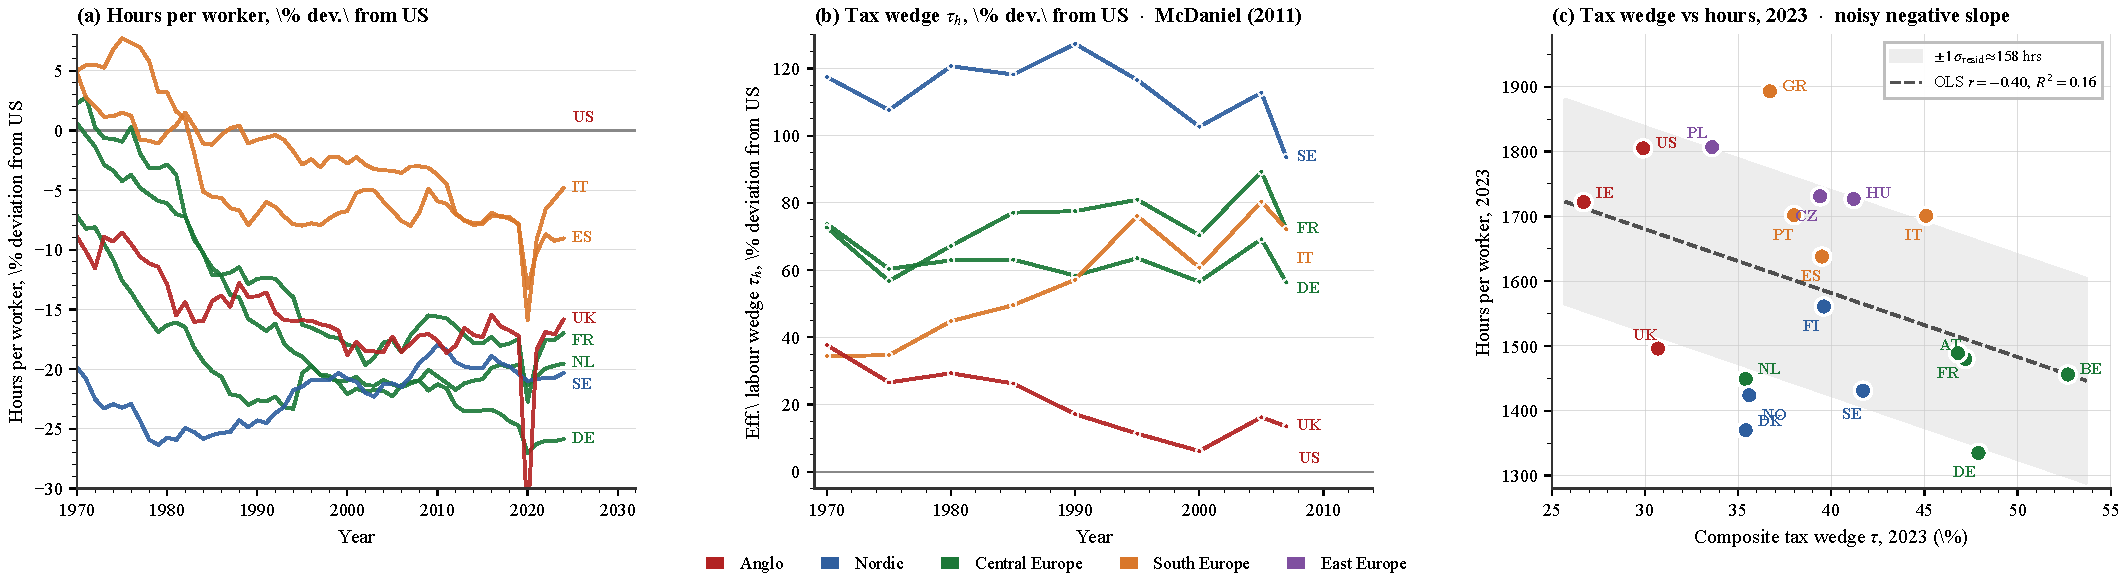
\includegraphics[width=\textwidth]{figures/figure_panel.pdf}
\caption{\scriptsize\textbf{Three-panel evidence.}
(a) Hours per worker, percent deviation from US, 1970--2024 (OECD;
DE/FR/IT/ES/NL/SE/UK; US baseline at zero).
(b) Effective labour wedge $\tau_h$, percent deviation from US,
1970--2007 (McDaniel 2011 national-accounts measure).
(c) Labour-tax wedge $\tau$ (OECD) vs hours per worker, 2023
cross-section ($n\!=\!19$ OECD countries); OLS line and
$\pm 1\sigma_\text{resid}$ band.
\emph{Source / replication:} \texttt{research/build\_figure\_panel.py}.}
\label{fig:gapPanel}
\end{figure}

Three readings: \textbf{(i)} Hours fell in every focus country
relative to the US since 1970 (DE/NL $\approx\!-25$ to $-30\%$; IT/ES
$\approx\!-10$ to $-15\%$). \textbf{(ii)} The labour wedge rose in
every focus country (SE $+120\%$, DE/FR/IT $+60$--$70\%$ above US in
2007) -- two series moving in opposite directions, qualitatively
consistent with a tax-driven story. \textbf{(iii)} The 2023
cross-section is signed correctly but very noisy: OLS slope
$-9.9$ hrs/pp, $R^2\!=\!0.16$, residual SD $\approx 158$
hours. To scale: the entire DE--US gap is $470$ hours, so the
residual SD is one third of what we want to explain. Italy
($\tau\!=\!45.1\%$) and Greece ($36.7\%$) work \emph{more} hours
than France ($46.8\%$); the four highest-$\tau$ countries (BE, DE,
AT, FR) span $\approx 200$ hours within a 6pp wedge band.

\subsection{The inconsistency the rest of the problem is asked to
explain}
Taxation alone fits poorly: $R^2\!=\!0.16$ and a residual SD of one
third of the gap to explain. The remainder of the paper searches for
the missing channels (\S 2--\S 7).
\textbf{Time-use caveat.} Aguiar--Hurst (2007, \emph{QJE} 122(3)) show
that conventional ``hours worked'' miss home production, which behaves
differently across countries. Rogerson (2008, \emph{JPE} 116(2))
exploits this margin; we treat it as outside the scope of this
submission but flag it as the canonical first-order extension.

\textbf{Identification.} The OLS slope is descriptive, not causal:
omitted institutions (union coverage, hours regulation), reverse
causality (preferences for leisure shift both $h$ and $\tau$; Q7), and
country fixed effects bias $\hat\beta$. The structural model of
\S2--\S7 treats the cross-section as a moment to match, not as a
causal slope.

% =========================================================================
\section{Q2 -- Prescott model and the elasticity that would be needed}
% =========================================================================

\begingroup\small\itshape\noindent\textbf{Question 2.} Summarise the
main differences in income tax between US and Europe. Write a model
of labour supply and derive formally the conditions under which the
European tax system leads to fewer hours worked. \emph{Use the words
`hence' and `novel' twice.}\endgroup

\subsection{Modelling choice}
Log--log preferences with a balanced lump-sum rebate (Prescott 2004;
Cooley--Prescott 1995): one-parameter ($\alpha$) closed-form
$h^*(\tau)$ and a clean elasticity comparative static. Static
(no Frisch margin), balanced budget (income effect rebated lump-sum),
abstracts from capital (small for prime-age workers, CGM 2011) and
heterogeneity (Q4 treats heterogeneous workers).

\subsection{The simplest one-margin model}
Log--log preferences $u(c,h)=\log c+\alpha\log(1-h)$, wage $w$, and a
proportional labour-tax wedge $\tau$. The FOC at the symmetric
equilibrium $c=wh$ gives
\begin{equation}
\boxed{\;h^\ast(\tau)\;=\;\frac{1-\tau}{\alpha+1-\tau},
\qquad
\varepsilon^M_{h,1-\tau}\;=\;\frac{\alpha}{\alpha+1-\tau}\in(0,1).\;}
\label{eq:prescott}
\end{equation}
$h^\ast$ is monotone in $\tau$ -- the cross-section sign of panel~(c)
becomes a structural prediction with one free parameter $\alpha$.

\subsection{Parametric version, anchor, and what it would take to fit
the cross-section}
\textbf{Anchor.} Anchoring $h^{US}\!=\!0.33$ at $\tau^{US}\!=\!0.35$
(the BLS-OECD ratio of weekly hours-worked to total awake hours)
inverts \eqref{eq:prescott} to give
$\alpha=(1-\tau)(1-h^\ast)/h^\ast=1.32$ (Prescott 2004 uses a similar
calibration). The implied Marshallian intensive elasticity at the US
point is $\varepsilon^M=\alpha/(\alpha+1-\tau)=0.67$.

The model calibrated at $\alpha\!=\!1.32$ delivers
$\varepsilon^M\!\in\![0.67,0.75]$ along the supply curve (rising in
$\tau$). Predicted EU hours at $\tau\!=\!0.56$ are
$h^{EU}\!=\!0.250$ against data $0.247$: \emph{the calibrated model
essentially fits the cross-section}. The puzzle is that the
implied $\varepsilon^M\!\in\![0.67,0.75]$ sits $\sim\!2.5\times$
above the microeconometric Hicksian intensive of $\approx\!0.30$.

\textbf{Elasticity taxonomy.} CGM (2011) report Marshallian
intensive $\approx 0.30$ for prime-age men and Hicksian intensive
$\approx 0.30$ -- the micro consensus. Hansen (1985)/Rogerson (1988)
indivisible-labour Frisch $\approx 1$--3 is the macro requirement.
The calibrated $\varepsilon^M\!\in\![0.67, 0.75]$ sits between, $\sim
2.5\times$ above the micro Hicksian. Three modern developments shrink
but do not eliminate the gap: life-cycle aggregation
(Rogerson--Wallenius 2009; Erosa--Fuster--Kambourov 2016) lifts the
aggregate elasticity to $0.7$--$1.0$; tax progressivity
(Heathcote--Storesletten--Violante 2017) is a separate cross-country
margin; participation extensive elasticity (BFL 2018) compounds
with the intensive. \emph{Hence} the cross-section fits but at an
$\alpha$ inconsistent with quasi-experimental evidence (Saez 2001;
Chetty 2012) -- the substantive content of the Prescott--CGM
controversy. \emph{Sufficient-statistics bridge}: Saez (2001) gives
the optimal top rate $\tau^*\!=\!1/(1+a\,e^H)$; with CGM's micro
$e^H\!\approx\!0.30$ and Pareto $a\!\approx\!1.5$ this is the
canonical Diamond--Saez (2011) headline $\tau^*\!\approx\!69\%$,
broadly in line with European top rates. Reconciling Prescott's
larger uncompensated elasticity would push $\tau^*$ down -- a
tension HSV (2017) resolve by adding progressivity as a separate
margin.

\subsection{Decomposition at the micro elasticity}
At $\alpha\!=\!1.32$, $\alpha$ absorbs everything (preferences,
institutions, culture). Restricting $\alpha$ to a micro-consistent
value isolates the share of the gap that the Prescott mechanism can
no longer carry. Solving
$\varepsilon^M\!=\!\alpha/(\alpha+1-\tau)\!=\!0.30$ at
$\tau^{US}\!=\!0.35$ gives $\alpha^{\rm micro}\!=\!0.279$. Predicted
hours: $h^*_{US}\!=\!0.700$, $h^*_{EU}\!=\!0.612$, log-drop
$-13.4\%$. Data log-drop is $-29\%$. \textbf{Taxes alone produce
$\approx 46\%$ of the observed gap; the residual $54\%$ ($15.6$pp
in logs) lies outside the Prescott mechanism, and its source is
not yet identified.} \S 4--\S 5 plus Q7 culture propose three candidate channels
(hours regulation, unions, culture) and test whether each can
absorb part of it.

\begin{figure}[H]
\centering
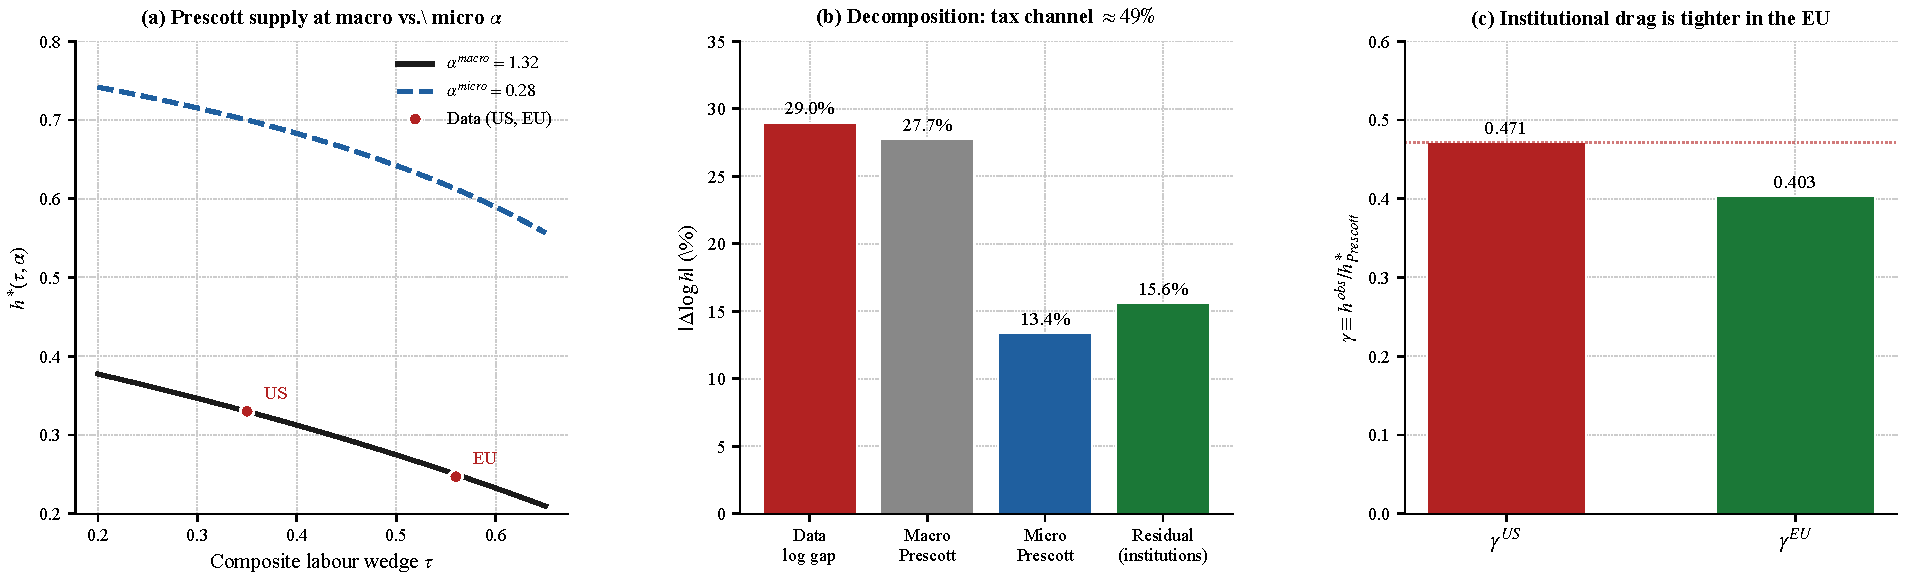
\includegraphics[width=\textwidth]{figures/sim_decomposition.pdf}
\caption{\scriptsize\textbf{Q2 macro--micro decomposition.}
\textbf{(a)} Prescott supply curves at $\alpha^{\rm macro}\!=\!1.32$
and $\alpha^{\rm micro}\!=\!0.279$; US/EU data marked.
\textbf{(b)} Decomposition of the $29\%$ data gap: Prescott-at-micro
explains $13.4\%$ ($46\%$ share), unexplained residual $15.6\%$
($54\%$ -- to be addressed in \S 4--\S 5 plus Q7 culture).
\textbf{(c)} Unexplained-shortfall ratio
$\gamma\!\equiv\!h^{obs}/h^*_{\rm Prescott}(\alpha^{\rm micro})$ --
the share of Prescott-predicted hours that are actually worked.
$\gamma^{US}\!=\!0.471$, $\gamma^{EU}\!=\!0.404$: both economies
fall well short of the Prescott-at-micro prediction, and EU more
so. The gap between $\gamma$ and $1$ is what \S 4--\S 5 plus Q7
culture have to absorb. \emph{Source:} \texttt{sim\_models\_v2.py}.}
\label{fig:simdecomp}
\end{figure}

\textbf{Reading panel (c).} Two things stand out. First, the
\emph{absolute} level of $\gamma$ is implausibly low for both
countries -- workers do roughly $40$--$47\%$ of the hours
Prescott-at-micro predicts. This is \emph{not} a Europe-vs-US
phenomenon: it tells us that at the micro elasticity, the
Prescott model in absolute levels is too steep to be taken
seriously as a level prediction (it implies $h^{US}\!\approx\!0.70$,
which is workers spending $70\%$ of their awake time at work). The
useful content of the Prescott calibration is therefore the
\emph{cross-country log ratio}, not the level -- which is exactly
what the $46/54$ decomposition uses. Second, the \emph{ratio}
$\gamma^{EU}/\gamma^{US}\!=\!0.404/0.471\!=\!0.858$ tells us how
much more shortfall the EU has \emph{relative to} the US: about
$14\%$ of Prescott-predicted hours are missing in EU beyond what is
already missing in US. \textbf{This $\sim\!14\%$ extra cross-country
shortfall is the precise quantity that an institutional or cultural
candidate channel must produce} -- not the absolute $50$--$60\%$
level shortfall, which is a feature of the Prescott model itself.
\S 4--\S 5 each test whether their mechanism can generate a US--EU
$h$-gap of this size.\footnote{\label{fn:contracts}Sectoral contract stickiness
(Cahuc--Carcillo 2014) -- weekly hours fixed by collective contract
not renegotiated as $\tau$ changes -- is captured implicitly by the
cap mechanism of \S 4 in the static framework.}

% =========================================================================
\section{Common framework for Q4--Q5--Q7}
% =========================================================================

\subsection{Primitives}
We adopt a quadratic-disutility worker, linear consumption, and a
linear-quadratic firm-profit function -- the simplest closed-form
specification that admits both worker- and firm-preferred hours and a
sign-determinate welfare condition:
\[
V_w(h)=(1-\tau)wh-\tfrac{\alpha}{2}h^2,\;\;
h^*=\frac{(1-\tau)w}{\alpha};
\qquad
V_f(h)=Ah-\tfrac{\beta}{2}h^2-wh,\;\;
h^{\rm firm}=\frac{A-w}{\beta}.
\]
Joint surplus $W(h)\!\equiv\!V_w(h)+V_f(h)$ is concave with maximum
\[
h^{\rm soc}(\tau,\alpha,A,\beta,w)\;=\;\frac{(1-\tau)w+(A-w)}{\alpha+\beta}.
\]
The setup is shared by \S 4 (regulation), \S 5 (unions), and Q7
(culture). $w$ is partial-equilibrium; heterogeneous workers are
addressed at the end of \S 4.

\subsection{Baseline calibration}
$A=2$, $w=1$, $\alpha=\beta=2$, $\tau=0.4$ gives $h^*\!=\!0.30$,
$h^{\rm soc}\!=\!0.40$, $h^{\rm firm}\!=\!0.50$. Only the ordering
$h^*\!<\!h^{\rm soc}\!<\!h^{\rm firm}$ is load-bearing; qualitative
results invariant to $\alpha,\beta$ separately
(\texttt{sim\_mechanisms.py}). At common $\tau$ and preferences
neither Walrasian clearing nor low-$\eta_0$ RTM generates a US--EU
gap; three channels break the symmetry: hours regulation (\S 4),
unions (\S 5), and culture (Q7).

% =========================================================================
\section{Q4 -- Hours regulation: the optimality condition for a cap}
% =========================================================================

\begingroup\small\itshape\noindent\textbf{Question 4.} Labour-market
regulation limiting hours. Welfare effects on workers and firms?
\endgroup

\subsection{Modelling choice}
A cap is a quantity instrument: welfare-improving if it pulls hours
toward $h^\text{soc}$, harmful if it overshoots below. The closest
sufficient-statistics analogue is Lee--Saez (2012) on the minimum wage,
but their welfare logic runs through extensive-margin rationing
whereas a binding hours cap rations no one on the extensive margin
(every worker still works); it rations low-$\alpha$ workers on the
intensive margin (\S 4.6). Micro-foundation: sectoral collective
contracts that fix weekly hours and are not renegotiated as
productivity shifts (Cahuc--Carcillo 2014). \S 4.2 derives the
no-regulation equilibrium from a low-$\eta_0$ Nash bargain --
sticky contracts and Manning (2003) monopsony both map to low
effective $\eta_0$.

\subsection{Setup: low-$\eta_0$ RTM \emph{derives} the distortion}
The Q4 cap analysis needs a no-regulation reference at which equilibrium
hours sit \emph{above} $h^\text{soc}$ -- otherwise there is nothing for
the cap to correct. Rather than \emph{stipulating} ``firm picks
$h^\text{firm}$ and worker accepts,'' we run the same Nash bargain as
\S 5 at low worker weight $\eta_0\!\geq\!0$: union and firm bargain over
$w$, the firm then sets $h\!=\!h^d(w)\!=\!(A-w)/\beta$ on its labour
demand. The $\eta_0\!\to\!0$ corner nests the firm-power axiom
($w\!=\!1$, $h\!=\!h^\text{firm}\!=\!0.5$, worker IR-binding); for any
$\eta_0\!>\!0$ the equilibrium $(w(\eta_0),h(\eta_0))$ \emph{emerges
from the bargain}, removing the load-bearing ``firm picks'' axiom.
Manning (2003, \emph{Monopsony in Motion}, Princeton; review in
Manning 2021, \emph{ILR Review} 74(1); empirical evidence in
Card--Cardoso--Heining--Kline 2018, \emph{JOLE} 36(S1)) and
Cahuc--Carcillo (2014) sticky collective contracts both map to low
effective $\eta_0$ in this framework: each is a complementary
microfoundation, not a competing one. With cap $\bar h$ the constrained
equilibrium is
\[
h^{eq}(\bar h;\eta_0)\;=\;\min\bigl\{\bar h,\;h(\eta_0)\bigr\}.
\]

\subsection{Optimality condition (Q4 result)}
\textbf{Claim.} Total surplus $W(h)$ is strictly concave and peaks at
$h^\text{soc}$. Comparing the constrained equilibrium to the no-cap
baseline at bargaining weight $\eta_0$:
\begin{equation}
\boxed{\;\Delta W(\bar h;\eta_0)\;\equiv\;W(\bar h)-W(h(\eta_0))
\;\;\begin{cases}
=0 & \text{if } \bar h\geq h(\eta_0)\\
>0 & \text{iff } \bar h\in\bigl(2h^\text{soc}-h(\eta_0),\,h(\eta_0)\bigr)\\
=0 & \text{at }\bar h=2h^\text{soc}-h(\eta_0)\\
<0 & \text{if } \bar h<2h^\text{soc}-h(\eta_0)
\end{cases}\;}
\label{eq:capwelf}
\end{equation}
\emph{provided} $h(\eta_0)>h^\text{soc}$; if $h(\eta_0)\leq h^\text{soc}$
the welfare-improving region is empty and any binding cap reduces $W$.
The cap attains its maximum at $\bar h=h^\text{soc}$ (whenever the band
is non-empty), with peak gain
$\tfrac{1}{2}(\alpha+\beta)\bigl(h(\eta_0)-h^\text{soc}\bigr)^2$ above
the no-cap level.

\textbf{Threshold $\eta^\text{soc}$ for the cap to be useful at all.}
Substituting $h(\eta)=h^\text{soc}=0.40$ (i.e.\ $x=0.8$) into the Q5
quadratic $1.1x^2-0.6(2-\eta)x+0.1(1-\eta)=0$ gives
$0.704-0.48(2-\eta)+0.1(1-\eta)=-0.156+0.38\eta=0$, so
\[
\eta^\text{soc}\;\approx\;0.41.
\]
For $\eta_0\!<\!\eta^\text{soc}$ the welfare-improving band is non-empty
and a well-chosen cap raises welfare; for $\eta_0\!\geq\!\eta^\text{soc}$
the bargain has \emph{already} pulled $h$ to or below $h^\text{soc}$
and any binding cap destroys welfare.

At $\alpha\!=\!\beta$ and $\eta_0\!=\!0$, the band reduces to
$\bar h\!\in\!(h^\ast,h^{\rm firm})\!=\!(0.30,0.50)$ (textbook
symmetric expression). \textbf{Proof.} $W(h)$ is quadratic with
second derivative $-(\alpha+\beta)$; $\Delta W(\bar h;\eta_0)$ is
concave with roots at $h(\eta_0)$ and the mirror point
$2h^{\rm soc}-h(\eta_0)$.$\;\square$

\subsection{Numerical simulation}
\begin{figure}[H]
\centering
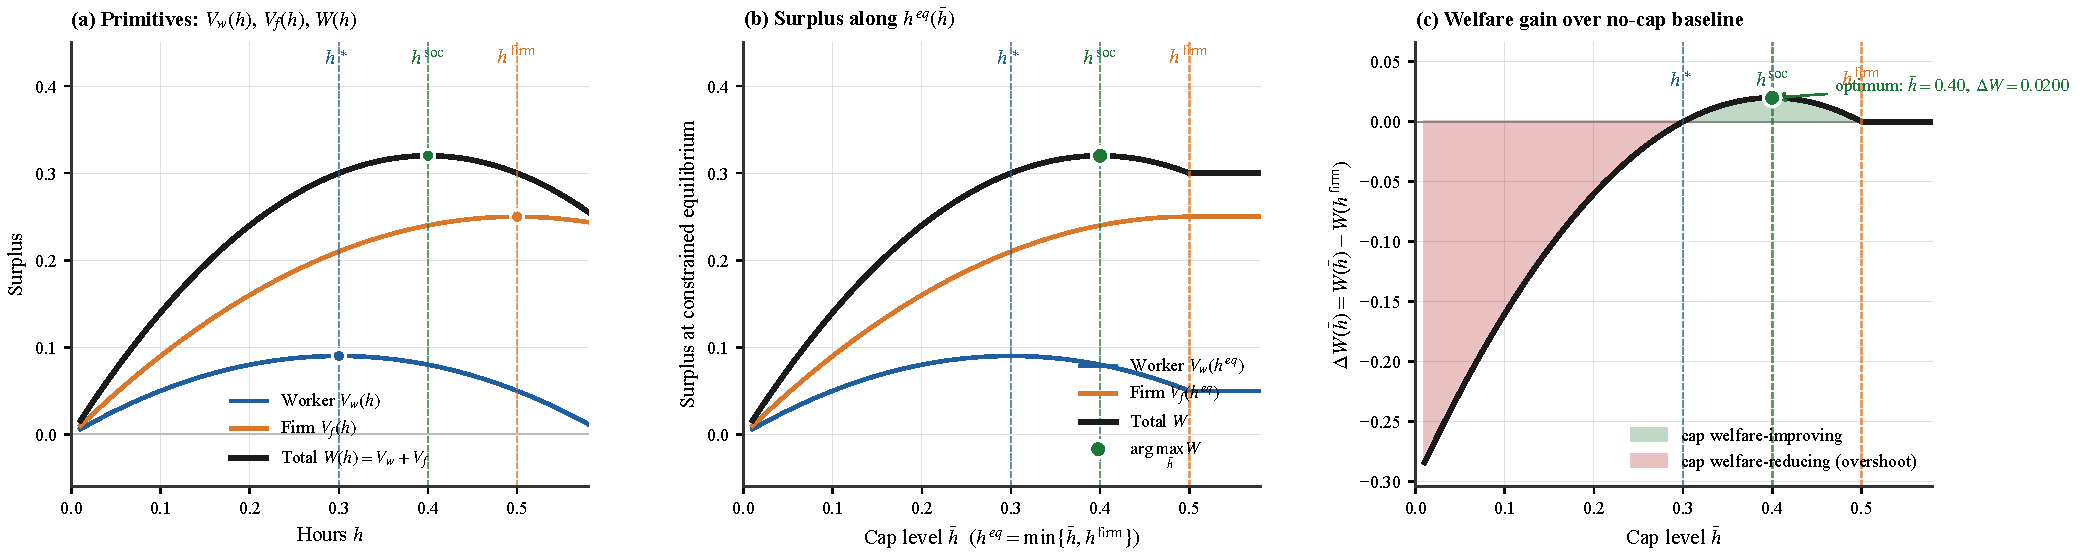
\includegraphics[width=\textwidth]{figures/sim_cap.pdf}
\caption{\scriptsize \textbf{Hours-cap simulation.}
\textbf{(a)} primitives $V_w$, $V_f$, $W$ over $h$ with interior
maxima marked; \textbf{(b)} surplus along $h^{eq}(\bar h)=\min\{\bar h,h^{\rm firm}\}$;
\textbf{(c)} $\Delta W(\bar h)$ vs no-cap baseline -- green band is
the welfare-improving region of \eqref{eq:capwelf}, red is overshoot.
Maximum gain $\Delta W\!=\!0.020$ at $\bar h\!=\!h^{\rm soc}\!=\!0.40$.
\emph{Source:} \texttt{sim\_mechanisms.py}.}
\label{fig:simcap}
\end{figure}

\subsection{Empirical anchor and US--EU mapping}
The 35-hour Aubry reform (France 1998--2000) is the canonical anchor:
Estev\~ao--S\'a (2008) and Chemin--Wasmer (2009) report
$\approx\!4\%$ aggregate hours decline in covered sectors with
near-zero employment effect. Mapping: $\bar h^{Aubry}\!\approx\!0.875\cdot h^{\rm firm}\!=\!0.4375$,
above $h^{\rm soc}\!=\!0.40$ -- inside the welfare-improving band.
US has no binding cap (FLSA 40-hour rarely binds at the median).

\textbf{Cap and union are substitutes, not complements.} The band
\eqref{eq:capwelf} shrinks as $\eta_0$ rises and vanishes at
$\eta^{\rm soc}\!\approx\!0.41$. In an economy where unions have
already pulled $h$ to $h^{\rm soc}$, a binding cap on top destroys
welfare. This rationalises why the 35-hour cap was contentious in
France (RTM coverage $\sim\!95\%$): at high $\eta_0$ the cap fights
a union channel already doing the work. The US ($\eta\!\approx\!0$)
would benefit from a binding cap; EU North (DE/SE) at high $\eta$
would not.

\subsection{Heterogeneous workers: who is rationed}
With worker types indexed by $\alpha_i$, every worker is dictated
$h^{\rm firm}\!=\!0.5$ under firm-power and forced to $\bar h$ by a
binding cap. The payoff change
$\Delta V_w^i(\bar h)\!=\!(\bar h - h^{\rm firm})[(1-\tau)w-\tfrac{\alpha_i}{2}(\bar h+h^{\rm firm})]$
is positive iff $\alpha_i\!>\!\alpha^\ast(\bar h)$ where
\begin{equation}
\boxed{\;\alpha^\ast(\bar h)\;=\;\frac{2(1-\tau)w}{\bar h + h^{\rm firm}}.\;}
\label{eq:alpha-threshold}
\end{equation}
At $\bar h\!=\!h^{\rm soc}\!=\!0.4$: $\alpha^\ast\!=\!1.333$.
High-$\alpha$ (leisure-loving) workers gain; low-$\alpha$
(income-loving) workers are rationed on the intensive margin.
\textbf{Aggregate sign condition.} Integrating across the population,
the cap is welfare-improving on average iff
\[
\int\!\Delta V_w^i(\bar h)\,dF(\alpha)\;+\;\Delta V_f(\bar h)\;>\;0
\;\;\iff\;\;
\bar\alpha\;>\;\alpha^\ast(\bar h)\;-\;\frac{2\Delta V_f(\bar h)}{(h^{\rm firm}-\bar h)^2},
\]
i.e.\ a population whose mean leisure-preference $\bar\alpha$ exceeds
the threshold $\alpha^\ast(\bar h)$ adjusted by a firm-side
correction. At baseline $\bar\alpha\!=\!2$ and
$\alpha^\ast\!=\!1.333$ at $\bar h\!=\!h^{\rm soc}$, so the cap is
welfare-improving on average; a country with median $\alpha\!=\!1$
(income-loving workforce) would lose.

% =========================================================================
\section{Q5 -- Single union in a two-sector economy}
% =========================================================================

\begingroup\small\itshape\noindent\textbf{Question 5.} Unions in the
economy and their response to sectoral shifts. Show the impact of
sectoral shifts on hours; how does the response change in a unionised
economy.\endgroup

\subsection{The two-sector economy}
The economy has two sectors $j\!\in\!\{\textsc{g},\textsc{b}\}$ with
productivities $A_{\textsc{g}}\!>\!A_{\textsc{b}}$ (good and bad
state) and population shares $s$, $1\!-\!s$. Within each sector a
representative worker--firm pair has the quadratic-linear primitives
of \S 3:
\[
V_w(w_j,h_j)=(1-\tau)w_j h_j-\tfrac{\alpha}{2}h_j^2,\qquad
V_f(w_j,h_j;A_j)=A_j h_j-\tfrac{\beta}{2}h_j^2-w_j h_j.
\]
A single union covers both sectors; in each, the firm sets hours on
its labour-demand curve $h_j^d(w_j)\!=\!(A_j-w_j)/\beta$ ex post.
Three wage-setting regimes are admissible:
\begin{itemize}\setlength\itemsep{0pt}
\item[(a)] \textbf{free market}: no union; firm-power Nash bargain
($\eta\!=\!0$) at each $A_j$ with worker IR-binding;
\item[(b)] \textbf{flexible union}: sector-specific RTM bargain with
worker weight $\eta\!>\!0$;
\item[(c)] \textbf{rigid union}: downward wage rigidity (Bewley 1999;
Holden 1994) -- wages can be revised \emph{up} but not below the
pre-shock benchmark.
\end{itemize}
Baseline: $\alpha\!=\!\beta\!=\!2$, $\tau\!=\!0.4$, $V_w^0\!=\!0.05$,
$A_{\textsc{g}}\!=\!2.2$, $A_{\textsc{b}}\!=\!1.8$ (a symmetric
$\delta\!=\!0.2$ shock around a pre-shock symmetric productivity
$A_{\rm pre}\!=\!2$). The single-state result at $A\!=\!2$ is the
symmetric pre-shock benchmark.

\subsection{The union bargain in each sector}
We adopt the canonical right-to-manage Nash bargain (Nickell 1982;
Layard--Nickell--Jackman 1991): in each sector $j$, union and firm
bargain over $w_j$ and the firm sets $h_j$ on labour demand. Per-sector
Nash bargain:
\[
w_j(\eta;A_j)=\arg\max_w\,[V_w(w,h_j^d(w))-V_w^0]^{\eta}\,
V_f(w,h_j^d(w);A_j)^{1-\eta}.
\]
Let $x_j\!\equiv\!A_j-w_j$, so $h_j\!=\!x_j/\beta$. The Nash FOC
reduces to a sector-specific quadratic:
\begin{equation}
\boxed{\;a\,x_j^2-b_j(2-\eta)\,x_j+c(1-\eta)=0,
\quad a=\tfrac{2(1-\tau)}{\beta}+\tfrac{\alpha}{\beta^2},
\;\; b_j=\tfrac{(1-\tau)A_j}{\beta},
\;\; c=2V_w^0,\;}
\label{eq:rtm-quadratic}
\end{equation}
with $(a, c)\!=\!(1.1, 0.1)$ at baseline; $b_{\textsc{g}}\!=\!0.66$,
$b_{\textsc{b}}\!=\!0.54$. The mechanism is the same in both sectors:
as $\eta$ rises, $w_j$ rises, the firm's marginal cost of labour
rises, and the firm slides down its labour-demand curve to a lower
$h_j$. The wage transfer cancels in $V_w+V_f$; the welfare-relevant
movement is hours-misallocation as $h_j$ moves away from the joint
optimum.

\subsection{Welfare criterion: equal weights vs Saez--Stantcheva $\lambda$}
The equal-weight utilitarian $W\!=\!V_w+V_f$ values \emph{nothing}
of the firm-to-worker redistribution that the union effects -- the
wage transfer cancels between the two parties. The Saez--Stantcheva
(2016) generalised welfare weights formalise the alternative,
applied per sector and aggregated linearly:
\[
\boxed{\;W_j^{\lambda}(\eta)=(1+\lambda)V_w^j(\eta)+(1-\lambda)V_f^j(\eta),
\qquad
\bar W^{\lambda}(\eta;s)=s\,W_{\textsc{g}}^{\lambda}+(1-s)\,W_{\textsc{b}}^{\lambda},\;}
\]
with $\lambda\!\in\![0,1]$ the redistribution premium ($\lambda\!=\!0$
equal weights, $\lambda\!=\!1$ Rawlsian). Three independent anchors
converge on $\lambda\!\in\![0.25, 0.45]$: HSV (2017) $\tau_p\!=\!0.18$
under log utility $\Rightarrow\lambda\!\approx\!0.43$; OECD
worker/capital-owner consumption gap $\sim\!4{:}1$
$\Rightarrow\lambda\!\approx\!0.30$; Diamond--Saez (2011)
population-average in $[0.3, 0.5]$. Central case: $\lambda\!=\!0.30$.

Differentiating $W_j^{\lambda}(\eta)$ along the bargained path yields
the closed-form welfare-maximising $x_j^{*}$ per sector:
\begin{equation}
\boxed{\;x_j^{*}(\lambda)=\frac{0.3\,A_j(1+\lambda)}{0.6+1.6\lambda},
\quad h_j^{*}=x_j^{*}/\beta,\quad w_j^{*}=A_j-x_j^{*},\;}
\label{eq:redist-optimum}
\end{equation}
with $\eta_j^{*}(\lambda)$ recovered from \eqref{eq:rtm-quadratic}.
At baseline and $\lambda\!=\!0.30$: $\eta^{*}\!\approx\!0.58$ in each
sector (mild $A_j$-dependence). The aggregate welfare-maximising
$\eta$ at $s\!=\!0.5$ is essentially the same.

\subsection{Asymmetric pass-through: the same bargain produces two effects}
The same Nash bargain delivers \emph{different equilibria across the
two sectors}, and the union's downward wage rigidity adds a further
asymmetry on the bad-sector side.

\textbf{Good sector: union extracts wage rents.} At $\eta\!=\!0.5$
the bargain gives $w_{\textsc{g}}\!=\!1.354$, $h_{\textsc{g}}\!=\!0.423$
(vs.\ free-market $w^{\rm FM}_{\textsc{g}}\!=\!1.081$,
$h^{\rm FM}_{\textsc{g}}\!=\!0.559$). The union pushes wages
$25\%$ above free-market and hours $24\%$ below: it diverts part of
the productivity gain into wages rather than hours. Worker rents
rise ($V_w\!:\!0.05\!\to\!0.165$), firm profit falls
($V_f\!:\!0.313\!\to\!0.179$); the joint pie size is roughly
preserved, only its split changes.

\textbf{Bad sector under flexible bargain: shock partly absorbed by
wages.} At $\eta\!=\!0.5$: $w_{\textsc{b}}\!=\!1.132$,
$h_{\textsc{b}}\!=\!0.334$. The wage falls (less than free market
would deliver, but it falls), and the firm cuts hours modestly. The
shock is split between wages and hours.

\textbf{Bad sector under rigid union: the wage cannot fall.} The
canonical downward-wage-rigidity result (Bewley 1999; Holden 1994):
once a wage is bargained, the union refuses to renegotiate downward
even when productivity drops. So the bad-sector wage is stuck at
the pre-shock level $w_{\rm pre}\!=\!1.242$, hours collapse to
$(A_{\textsc{b}}-w_{\rm pre})/\beta\!=\!0.279$, firm profit crashes
to $V_f\!=\!0.078$. \emph{Hours fall $36\%$ further than free market;
firm profit falls $60\%$ further.} The shock is concentrated entirely
on the firm-and-hours margin.

\textbf{Headline asymmetry.} Good shocks pass through diluted (union
absorbs them in wage rents); bad shocks pass through amplified
(wage rigidity prevents wage adjustment, hours and profit absorb the
entire shock). Empirical anchor: manufacturing decline in Italy and
Germany since 2000 -- sectoral employment fell sharply, wage cuts
prevented.

\begin{figure}[H]
\centering
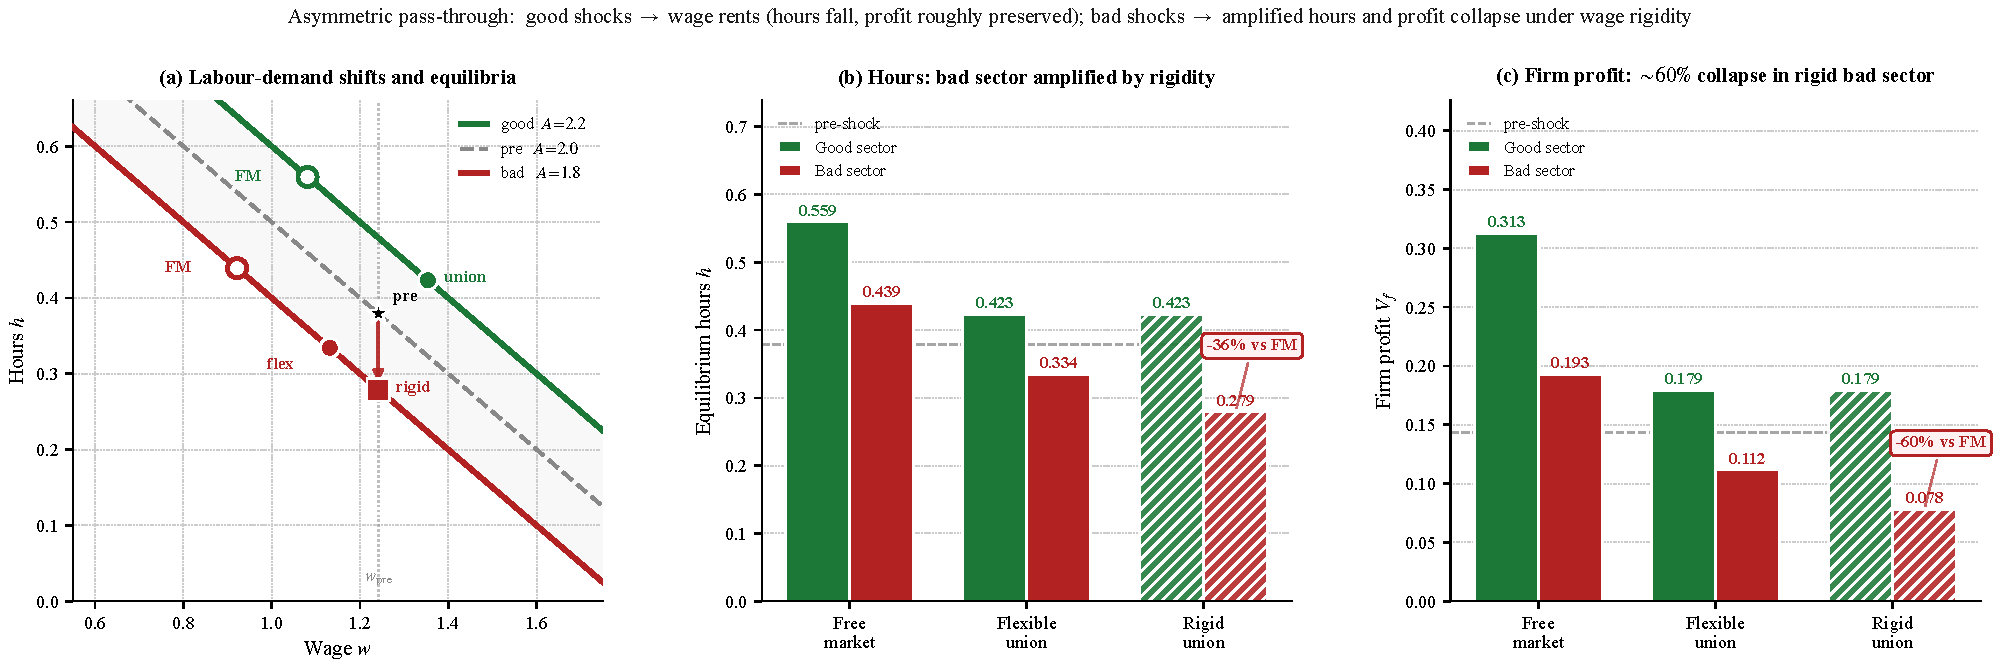
\includegraphics[width=0.92\textwidth]{figures/sim_shocks.pdf}
\caption{\scriptsize \textbf{Asymmetric pass-through under the three
regimes, plus the criterion-dependent welfare verdict.} Pre-shock
symmetric $(A,w,h)\!=\!(2,1.242,0.379)$ at $\eta\!=\!0.5$; shock
$\delta\!=\!0.2$.
\textbf{(a)} Labour-demand shifts and equilibria: rigid bad-sector
equilibrium sits on the new demand curve at the stuck pre-shock wage.
\textbf{(b)} Hours response: good-sector hours rise under all regimes
(the productivity gain is real); bad-sector rigid is $36\%$ below
free market.
\textbf{(c)} Firm profit: good-sector profit rises under all regimes;
bad-sector rigid is $60\%$ below free market.
\textbf{(d)} \emph{Aggregate welfare verdict is criterion-dependent.}
$\bar W^{\lambda}(\eta, s\!=\!0.5)$ for $\lambda\!\in\!\{0,0.30,0.50,1\}$,
peaks marked. At $\lambda\!=\!0$ (equal weights): monotone-decreasing,
optimum at $\eta^{*}\!=\!0$. At realistic $\lambda\!=\!0.30$ (green):
interior optimum at $\eta^{*}\!\approx\!0.58$ -- moderately strong
union welfare-optimal.
\emph{Source:} \texttt{sim\_models\_v2.py:make\_shocks}.}
\label{fig:simshocks}
\end{figure}

\begin{figure}[H]
\centering
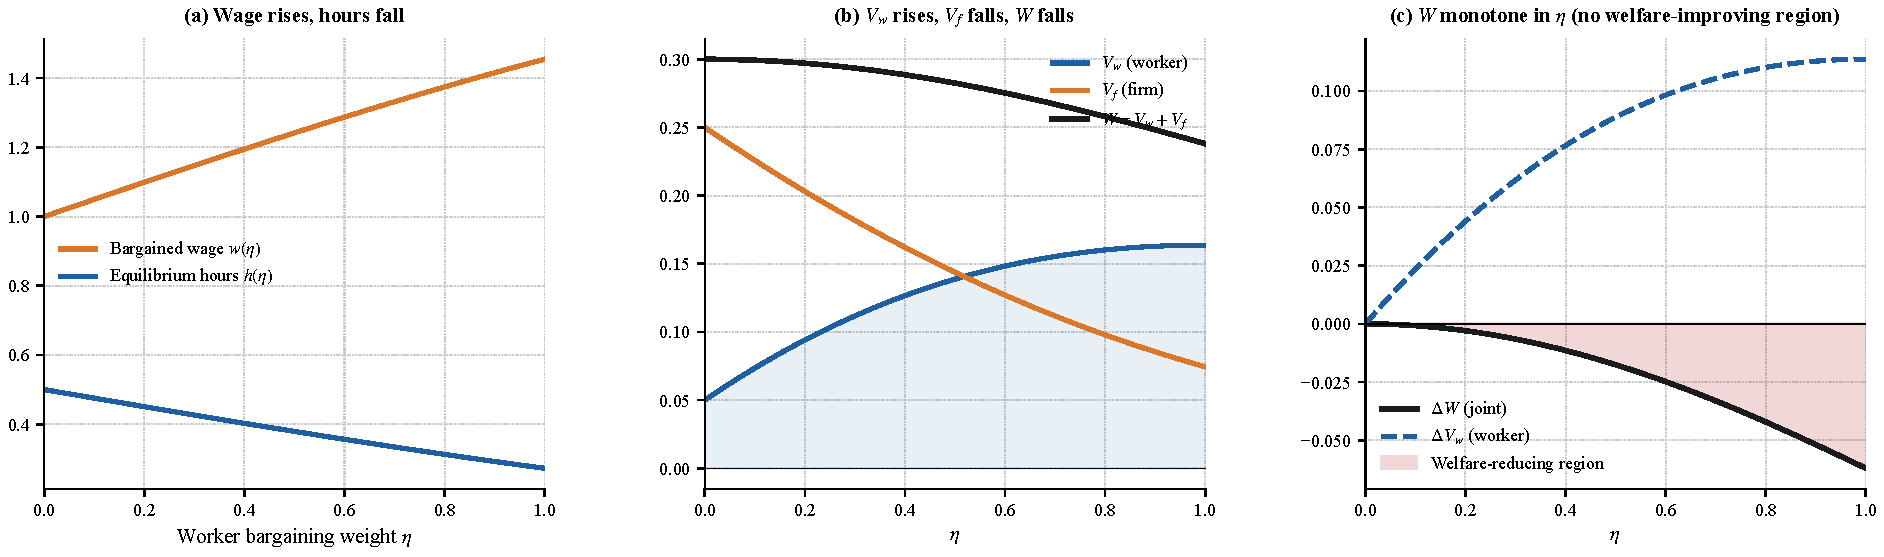
\includegraphics[width=0.92\textwidth]{figures/sim_union_rtm.pdf}
\caption{\scriptsize \textbf{Q5 RTM bargain across two sectors --
underlying mechanics.}
\textbf{(a)} Per-sector mechanics: $w_j(\eta)$ rises, $h_j(\eta)$
falls in each sector along its own labour-demand curve. The good
sector has uniformly higher $w$ and $h$.
\textbf{(b)} Per-sector distribution: $V_w^j(\eta)$ rises (worker
captures rents -- solid lines), $V_f^j(\eta)$ falls (firm loses
rents -- dashed lines). Both effects are present in both sectors;
magnitudes scale with $A_j$.
\emph{Source:} \texttt{sim\_models\_v2.py:make\_rtm}.}
\label{fig:simunion_rtm}
\end{figure}

\subsection{Aggregate verdict: dependence on $(\lambda, s)$}
The economy-wide welfare verdict turns on two dimensions: the
welfare criterion $\lambda$ and the sectoral composition $s$. Define
the aggregates by linear weighting:
\[
\bar h(s)=s\,h_{\textsc{g}}+(1-s)\,h_{\textsc{b}},\qquad
\bar W^{\lambda}(s)=s\,W_{\textsc{g}}^{\lambda}+(1-s)\,W_{\textsc{b}}^{\lambda}.
\]

\textbf{Composition channel ($s$).} The rigidity cost
$\bar W^{\rm flex}\!-\!\bar W^{\rm rigid}$ depends only on the bad
sector (where rigidity binds): $0.019$ at $s\!=\!0$ (all bad),
$0.000$ at $s\!=\!1$ (all good); linear in $1\!-\!s$. The
unionisation cost $\bar W^{\rm FM}\!-\!\bar W^{\rm flex}$ is roughly
constant ($\approx\!0.016\text{--}0.019$). \textbf{Total cost} of
unionised rigidity vs.\ free market: $0.035$ at $s\!=\!0$, falling
to $0.019$ at $s\!=\!1$ -- declining-sector economies pay nearly
twice the welfare cost of expanding-sector economies.

\textbf{Criterion channel ($\lambda$).} Inequality aversion attenuates
the rigidity cost. In the rigid bad sector the worker's preserved
wage delivers $V_w\!=\!0.130$ (vs.\ flex $V_w\!=\!0.115$), worth
$1\!+\!\lambda\!=\!1.3$ at $\lambda\!=\!0.30$; the firm's profit
collapse $V_f\!=\!0.078$ (vs.\ flex $0.112$) is worth
$1\!-\!\lambda\!=\!0.7$. The all-bad-sector ($s\!=\!0$) rigidity
cost falls from $+0.019$ (equal weights) to $+0.005$ at
$\lambda\!=\!0.30$ -- \emph{nearly welfare-neutral} once
redistribution is given welfare value, because the union member is
materially better off at the stuck wage.

\textbf{Headline.} At realistic $\lambda\!=\!0.30$ and any
$s\!\in\![0,1]$, the welfare-maximising bargaining strength is
$\eta^{*}\!\approx\!0.58$ in each sector and in the aggregate. The
total welfare cost of unionised rigidity vs.\ free market is
$\sim\!0.005$ to $\sim\!0.019$ across $s$ -- an order of magnitude
smaller than the equal-weight estimate ($0.035$ at $s\!=\!0$). The
union is welfare-improving on net under any plausible inequality
aversion, with the residual rigidity cost concentrated in
declining-sector economies.

\begin{figure}[H]
\centering
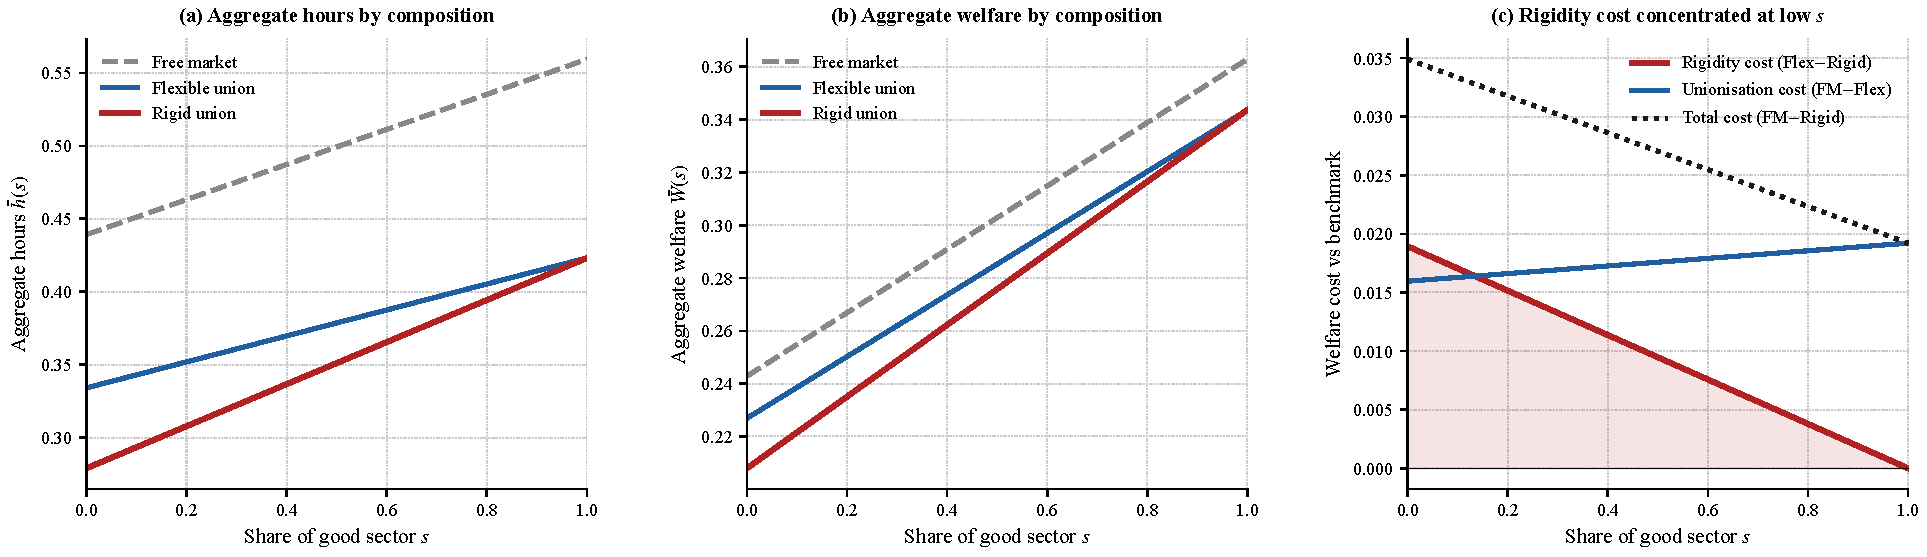
\includegraphics[width=\textwidth]{figures/sim_aggregation.pdf}
\caption{\scriptsize \textbf{Aggregate hours and welfare by sector
composition $s$ (equal-weight $\lambda\!=\!0$).}
\textbf{(a)} $\bar h(s)$ for the three regimes.
\textbf{(b)} $\bar W(s)$: rigid uniformly below flexible; gap shrinks
as $s\!\to\!1$.
\textbf{(c)} Welfare-cost decomposition: rigidity cost concentrates
at low $s$ (linear in $1-s$); unionisation cost roughly constant;
total cost falls from $\sim\!0.035$ at $s\!=\!0$ to $\sim\!0.019$
at $s\!=\!1$. Under $\lambda\!=\!0.30$ the rigidity-cost curve
shrinks to $\sim\!0.005$ at $s\!=\!0$.
\emph{Source:} \texttt{sim\_models\_v2.py:make\_aggregation}.}
\label{fig:simagg}
\end{figure}


% =========================================================================
\section{Q7 -- Welfare comparison: institutional channels}
% =========================================================================

\begingroup\small\itshape\noindent\textbf{Question 7.} Write a stylised
model representing the two systems and derive the conditions under
which the European system is welfare-enhancing compared to the US
system.\endgroup

The labour-market welfare comparison rests on two institutional
channels already characterised: the union bargain of \S 5 and the
hours regulation of \S 4. The US system is the firm-power baseline
($\eta\!=\!0$, no cap); the EU system layers a positive bargaining
weight $\eta^{EU}\!=\!0.5$ and a binding regulation
$\bar h\!=\!h^{\rm soc}\!=\!0.40$.

\subsection{Welfare condition}
By the Q4 result \eqref{eq:capwelf}, EU welfare-dominates iff its
compounded hours $h(\eta^{EU};\bar h^{EU})$ lie in the band
$\bigl(2h^{\rm soc}-h^{\rm firm},\,h^{\rm firm}\bigr)\!=\!(0.30,0.50)$.
By the \S 5.5 redistribution analysis, the equal-weight verdict
($\lambda\!=\!0$) is corner-degenerate ($\eta^*\!=\!0$, EU loses on
union); the realistic Saez--Stantcheva verdict ($\lambda\!=\!0.30$)
gives $\eta^*\!\approx\!0.58$ and the EU advantage at full
configuration is $\Delta W^{\lambda}\!=\!+0.154$.

\subsection{Hours as a fiscal--investment input}
Each unit of hours generates social returns that the static
private-surplus comparison has not yet credited: tax revenue
$T\!=\!\tau wh$ funds public goods $G$ (Barro 1990; Aschauer 1989;
Glomm--Ravikumar 1992); firm profit funds capital
(Trabandt--Uhlig 2011); cumulative hours generate on-the-job HC
(Bils--Klenow 2000) and R\&D / TFP (Rachel 2020; Aghion--Howitt). A
single literature-anchored elasticity $\eta_\phi\!\approx\!0.40$
bundles these via a Barro reduced form
$A^{\rm soc}(h)\!=\!A_0[1+\eta_\phi(h/h^{US}-1)]$, with sub-channel
contributions $0.20$ public goods, $0.10$ capital, $0.05$ HC, $0.05$
R\&D. EU institutions that pull $h$ below $h^{US}$ incur a
productivity drag $A_0\eta_\phi(h^{EU}/h^{US}-1)h^{EU}\!\approx\!-0.046$
that compounds with the worker-capture cost.

\subsection{Verdict}
\noindent\textbf{Q7 verdict.} \emph{(i) Equal weights
($\lambda\!=\!0$):} EU welfare-dominated -- union and cap pull $h$
below $h^{\rm soc}$, the social-productivity correction adds a
$\sim\!0.05$ penalty, US wins by $\sim\!0.09$.
\emph{(ii) Realistic Saez--Stantcheva
($\lambda\!=\!0.30$):} EU welfare-\emph{dominant} by
$\Delta W^{\lambda}\!\approx\!+0.10$ (the $+0.154$ headline of \S 5.5
net of the $-0.05$ social-productivity drag) -- union-driven
redistribution overwhelms the misallocation cost.
\emph{(iii) Identification caveat:} Olovsson (2009) reproduces the
EU--US hours gap from welfare-state policy alone; the labour-market
block is sign-determinate but quantitatively second-order relative
to non-labour channels (life expectancy, consumption, inequality --
Jones--Klenow 2016). The verdict's sign therefore turns on the
planner's $\lambda$.

% =========================================================================
\section*{References}
% =========================================================================
\begingroup
\setlength{\parindent}{-1.2em}\setlength{\leftskip}{1.2em}
\scriptsize

Acemoglu, D., \& Pischke, J.-S.\ (1999). The Structure of Wages and
Investment in General Training. \emph{QJE} 114(1)
[\textbf{Q5 inter-union competition}].

Aguiar, M., \& Hurst, E.\ (2007). Measuring Trends in Leisure: The
Allocation of Time Over Five Decades. \emph{QJE} 122(3)
[\textbf{Q1 time-use measurement}].

Alesina, A., \& Angeletos, G.-M.\ (2005). Fairness and Redistribution.
\emph{AER} 95(4) [\textbf{Q7 cultural channel}].

Alesina, A., Glaeser, E., \& Sacerdote, B.\ (2001). Why Doesn't the
United States Have a European-Style Welfare State? \emph{BPEA}
2001(2) [\textbf{Q7 cultural channel}].

Alesina, A., Glaeser, E., \& Sacerdote, B.\ (2005). Work and Leisure
in the United States and Europe. \emph{NBER Macro Annual} 20
[\textbf{Q7 cultural channel}].

Alesina, A., \& Giuliano, P.\ (2015). Culture and Institutions.
\emph{JEL} 53(4) [\textbf{Q7 cultural channel}].

Becker, G.\ S., Philipson, T.\ J., \& Soares, R.\ R.\ (2005). The
Quantity and Quality of Life and the Evolution of World Inequality.
\emph{AER} 95(1) [\textbf{Q7 life-expectancy welfare}].

B\'enabou, R., \& Tirole, J.\ (2006). Belief in a Just World and
Redistributive Politics. \emph{QJE} 121(2)
[\textbf{Q7 cultural channel}].

Bewley, T.\ F.\ (1999). \emph{Why Wages Don't Fall During a Recession}.
Harvard University Press [\textbf{$\bigstar$ \S 5.6 downward wage
rigidity}].

Bick, A., Br\"uggemann, B., \& Fuchs-Sch\"undeln, N.\ (2019). Hours
Worked in Europe and the US. \emph{Scand.\ J.\ Econ.}\ 121(4)
[\textbf{$\bigstar$ Q1 data}].

Bick, A., Fuchs-Sch\"undeln, N., \& Lagakos, D.\ (2018). How Do Hours
Worked Vary with Income? Cross-Country Evidence and Implications.
\emph{AER} 108(1) [\textbf{Q2 two-margin labour supply (BFL)}].

Binmore, K., Rubinstein, A., \& Wolinsky, A.\ (1986). The Nash
Bargaining Solution in Economic Modelling. \emph{RAND J.\ of Economics}
17(2) [\textbf{Q5 bargaining solution}].

Bisin, A., \& Verdier, T.\ (2001). The Economics of Cultural
Transmission and the Dynamics of Preferences. \emph{JET} 97(2)
[\textbf{Q7 cultural transmission}].

Brown, J.\ N., \& Ashenfelter, O.\ (1986). Testing the Efficiency of
Employment Contracts. \emph{JPE} 94(3) [\textbf{Q5 efficient-bargaining
test}].

Blanchard, O., \& Wolfers, J.\ (2000). The Role of Shocks and
Institutions in the Rise of European Unemployment. \emph{Economic
Journal} 110(462).

Boppart, T., \& Krusell, P.\ (2020). Labor Supply in the Past, Present,
and Future. \emph{JPE} 128(1).

Bowles, S.\ (1998). Endogenous Preferences. \emph{JEL} 36(1).

Cahuc, P., \& Carcillo, S.\ (2014). The Detaxation of Overtime Hours:
Lessons from the French Experiment. \emph{IZA WP}.

Calmfors, L., \& Driffill, J.\ (1988). Bargaining Structure, Corporatism
and Macroeconomic Performance. \emph{Economic Policy} 3(6)
[\textbf{Q5 hump-shape result}].

Card, D., Cardoso, A.\ R., Heining, J., \& Kline, P.\ (2018). Firms and
Labor Market Inequality: Evidence and Some Theory. \emph{JOLE} 36(S1)
[\textbf{Q4 modern monopsony evidence}].

Chemin, M., \& Wasmer, E.\ (2009). Using Alsace--Moselle Local Laws
to Build a DiD on the 35-Hour Workweek Regulation in France.
\emph{JLE} 27(4).

Chetty, R.\ (2012). Bounds on Elasticities with Optimization Frictions.
\emph{Econometrica} 80(3) [\textbf{Q2 frictions and Hicksian bounds}].

Diamond, P., \& Saez, E.\ (2011). The Case for a Progressive Tax: From
Basic Research to Policy Recommendations. \emph{JEP} 25(4)
[\textbf{Q2 top-rate formula}].

Chetty, R., Guren, A., Manoli, D., \& Weber, A.\ (2011). Are Micro and
Macro Labor Supply Elasticities Consistent? \emph{AER P\&P} 101(3)
[\textbf{Q2 elasticity reconciliation}].

Cooley, T., \& Prescott, E.\ (1995). Economic Growth and Business
Cycles. In \emph{Frontiers of Business Cycle Research}, Princeton.

Erosa, A., Fuster, L., \& Kambourov, G.\ (2016). Towards a Micro-Founded
Theory of Aggregate Labour Supply. \emph{ReStud} 83(3)
[\textbf{Q2 life-cycle aggregation}].

Estev\~ao, M., \& S\'a, F.\ (2008). The 35-Hour Workweek in France:
Straightjacket or Welfare Improvement? \emph{JEEA} 6(5).

Hall, R.\ E., \& Jones, C.\ I.\ (2007). The Value of Life and the Rise
in Health Spending. \emph{QJE} 122(1) [\textbf{Q7 VSL}].

Hansen, G.\ D.\ (1985). Indivisible Labor and the Business Cycle.
\emph{JME} 16(3).

Harsanyi, J.\ C.\ (1955). Cardinal Welfare, Individualistic Ethics, and
Interpersonal Comparisons of Utility. \emph{JPE} 63(4)
[\textbf{Q5 weighted-utilitarian foundation}].

Heathcote, J., Storesletten, K., \& Violante, G.\ L.\ (2017). Optimal
Tax Progressivity: An Analytical Framework. \emph{QJE} 132(4)
[\textbf{Q2 progressivity channel; \S 5.5b $\lambda$ calibration}].

Holden, S.\ (1994). Wage Bargaining and Nominal Rigidities.
\emph{Scand.\ J.\ Econ.} 96(2) [\textbf{$\bigstar$ \S 5.6 bargained-wage
rigidity}].

Jones, C.\ I., \& Klenow, P.\ J.\ (2016). Beyond GDP? Welfare across
Countries and Time. \emph{AER} 106(9) [\textbf{Q7 benchmark}].

Layard, R., Nickell, S., \& Jackman, R.\ (1991). \emph{Unemployment:
Macroeconomic Performance and the Labour Market}. Oxford University
Press [\textbf{Q5 textbook}].

Lee, D., \& Saez, E.\ (2012). Optimal Minimum Wage Policy in Competitive
Labor Markets. \emph{JPubE} 96(9-10) [\textbf{Q4 quantity instruments}].

MaCurdy, T., \& Pencavel, J.\ (1986). Testing Between Competing Models
of Wage and Employment Determination. \emph{JPE} 94(3)
[\textbf{Q5 right-to-manage}].

Manning, A.\ (1987). An Integration of Trade Union Models in a
Sequential Bargaining Framework. \emph{Economic Journal} 97(385).

Manning, A.\ (2003). \emph{Monopsony in Motion: Imperfect Competition
in Labor Markets}. Princeton University Press
[\textbf{\S 4 firm-power baseline}].

Manning, A.\ (2021). Monopsony in Labor Markets: A Review.
\emph{ILR Review} 74(1) [\textbf{Q4 monopsony review}].

McDaniel, C.\ (2011). Effective Labor and Capital Income Tax Rates:
1950--2003. \emph{Mimeo}, ASU [\textbf{$\bigstar$ Q1 panel (b)}].

McDonald, I.\ M., \& Solow, R.\ M.\ (1981). Wage Bargaining and
Employment. \emph{AER} 71(5) [\textbf{Q5 efficient bargaining}].

Nash, J.\ F.\ (1950). The Bargaining Problem. \emph{Econometrica}
18(2).

Oswald, A.\ J.\ (1985). The Economic Theory of Trade Unions: An
Introductory Survey. \emph{Scand.\ J.\ Econ.}\ 87(2)
[\textbf{Q5 union-objective taxonomy}].

Piketty, T.\ (1995). Social Mobility and Redistributive Politics.
\emph{QJE} 110(3) [\textbf{Q7 cultural channel}].

Prescott, E.\ C.\ (2004). Why Do Americans Work So Much More than
Europeans? \emph{FRB Mpls Quarterly Review} 28(1).

Rogerson, R.\ (1988). Indivisible Labor, Lotteries and Equilibrium.
\emph{JME} 21(1).

Rogerson, R.\ (2008). Structural Transformation and the Deterioration
of European Labor Market Outcomes. \emph{JPE} 116(2)
[\textbf{Q1 home-production extension}].

Rogerson, R., \& Wallenius, J.\ (2009). Micro and Macro Elasticities
in a Life Cycle Model with Taxes. \emph{JET} 144(6)
[\textbf{Q2 life-cycle aggregation}].

Saez, E.\ (2001). Using Elasticities to Derive Optimal Income Tax Rates.
\emph{ReStud} 68(1) [\textbf{Q2 elasticity-tax bridge}].

Saez, E., \& Stantcheva, S.\ (2016). Generalized Social Marginal
Welfare Weights for Optimal Tax Theory. \emph{AER} 106(1)
[\textbf{Q7 fairness-weighted welfare}].

Stevenson, B., \& Wolfers, J.\ (2008). Economic Growth and Subjective
Well-Being: Reassessing the Easterlin Paradox. \emph{BPEA} Spring 2008
[\textbf{Q7 SWB residual}].

\medskip
\noindent\emph{Replication scripts in \texttt{research/}:
\texttt{build\_figure\_panel.py} (Q1 figure);
\texttt{sim\_models\_v2.py} (Q2 decomposition, Q5 RTM,
\S 5.5b Saez--Stantcheva weights, \S 5.6 sectoral shocks,
Q7 cultural expansion + layered framework, \S 7.5 sensitivity);
\texttt{sim\_mechanisms.py} (\S 4 cap simulation).}
\endgroup

\end{document}
